\documentclass[a4paper, 12pt]{article}

\usepackage[ngerman]{babel}
\usepackage[pages=all, color=black, position={current page.south}, placement=bottom, scale=1, opacity=1, vshift=5mm]{background}
\usepackage[margin=1in]{geometry} % full-width
\usepackage{setspace}

% SQL listings
\usepackage{xcolor,listings}
\usepackage{textcomp}
\usepackage{color}

\definecolor{codegreen}{rgb}{0,0.6,0}
\definecolor{codegray}{rgb}{0.5,0.5,0.5}
\definecolor{codepurple}{HTML}{C42043}
\definecolor{backcolour}{HTML}{F2F2F2}
\definecolor{bookColor}{cmyk}{0,0,0,0.90}  
\color{bookColor}

\lstset{upquote=true}

\lstdefinestyle{SQLstyle}{
    backgroundcolor=\color{backcolour},   
    commentstyle=\color{codegreen},
    keywordstyle=\color{codepurple},
    numberstyle=\numberstyle,
    stringstyle=\color{codepurple},
    basicstyle=\footnotesize\ttfamily,
    breakatwhitespace=false,
    breaklines=true,
    captionpos=b,
    keepspaces=true,
    numbers=left,
    numbersep=10pt,
    showspaces=false,
    showstringspaces=false,
    showtabs=false,
}



\lstset{style=SQLstyle}

\newcommand\numberstyle[1]{%
    \footnotesize
    \color{codegray}%
    \ttfamily
    \ifnum#1<10 0\fi#1 |%
}

\newcommand\SQL{[language=SQL,
	                    deletekeywords={IDENTITY},
	                    deletekeywords={[2]INT},
	                    morekeywords={clustered},
	                    framesep=8pt,
	                    xleftmargin=40pt,
	                    framexleftmargin=40pt,
	                    frame=tb,
	                    framerule=0pt]}

% AMS Packages
\usepackage{amsmath}
\usepackage{amsthm}
\usepackage{amssymb}

% Unicode
\usepackage[utf8]{inputenc}
\usepackage{hyperref}
\hypersetup{
	unicode,
%	colorlinks,
%	breaklinks,
%	urlcolor=cyan, 
%	linkcolor=blue, 
	pdfauthor={Frederik Folkers},
	pdftitle={A simple article template},
	pdfsubject={A simple article template},
	pdfkeywords={article, template, simple},
	pdfproducer={LaTeX},
	pdfcreator={pdflatex}
}

% BibLaTeX
\usepackage[
backend=biber,
style=alphabetic,
sorting=ynt
]{biblatex}
\addbibresource{Facharbeit.bib}

% Theorem, Lemma, etc
\theoremstyle{plain}
\newtheorem{theorem}{Theorem}
\newtheorem{corollary}[theorem]{Corollary}
\newtheorem{lemma}[theorem]{Lemma}
\newtheorem{claim}{Claim}[theorem]
\newtheorem{axiom}[theorem]{Axiom}
\newtheorem{conjecture}[theorem]{Conjecture}
\newtheorem{fact}[theorem]{Fact}
\newtheorem{hypothesis}[theorem]{Hypothesis}
\newtheorem{assumption}[theorem]{Assumption}
\newtheorem{proposition}[theorem]{Proposition}
\newtheorem{criterion}[theorem]{Criterion}
\theoremstyle{definition}
\newtheorem{definition}[theorem]{Definition}
\newtheorem{example}[theorem]{Example}
\newtheorem{remark}[theorem]{Remark}
\newtheorem{problem}[theorem]{Problem}
\newtheorem{principle}[theorem]{Principle}

\usepackage{graphicx, wrapfig, color}
\graphicspath{{fig/}}

%\usepackage[linesnumbered,ruled,vlined,commentsnumbered]{algorithm2e} % use algorithm2e for typesetting algorithms
\usepackage{algorithm, algpseudocode} % use algorithm and algorithmicx for typesetting algorithms
\usepackage{mathrsfs} % for \mathscr command

\usepackage{lipsum}

% Author info
\title{\small Facharbeit zum Thema: \\ \Large Zur Entwicklung und Implementation einer Datenbank anhand einer Schulkursbelegung}
%\author{Frederik Folkers}

\date{

}

\begin{document}
	\maketitle
	
	
	\begin{center}
	\vspace{3cm}
	\begin{tabular}{ll}
	Schule: & Gymnasium Verl \\
	Schuljahr: & 2021/2022\\
	Kurs: & Grundkurs Informatik\\
	Betreuender Lehrer: & Herr Jansen\\
	\end{tabular} 
	\vfill
	Vorgelegt von:\\
	Frederik Folkers
	\end{center}
	\newpage
	\tableofcontents	
	\vspace{1cm}
	Literaturverzeichnis\\
	Schlusserklärung\\
	Anhang liegt im USB-Stick bei (UI-Script, Datenabank, Vorbereitungsdateien)
	\newpage	
	
	\onehalfspace
	\section{Einleitung}
	\label{sec:intro}
	Im heutigen Informationszeitalter ist es wichtig, große und komplexe Datenmengen effizient abzuspeichern und die gewünschten Informationen strukturiert abrufen zu können. Daher habe ich für diese Facharbeit das Thema Datenbanken gewählt. \\
	Zunächst werde ich verschiedene Möglichkeiten zur Sicherung von Daten vorstellen, dann dieses Wissen exemplarisch am Beispiel einer Schulkursbelegung für die Oberstufe darstellen.
	
	\section{Allgemeine Informationen}
	\label{sec:allgInfo}
	
	\subsection{Datenbank Modelle}
	\label{sec:dbMod}
	Es gibt verschiedene Datenbankmodelle. Diese unterscheiden sich in ihrer Struktur und Funktionsweise. Die drei Wichtigsten werden in den nächten Abschnitten vorgestellt.
	
	\subsubsection{Hierarchisch}
	\label{sec:hierdb}
	
	\begin{wrapfigure}{r}{4cm}
	\vspace{-13pt}
	\includegraphics[width=4cm]{vertretungTree.png}
	\vspace{-30pt}
	\caption{Vertre\-tungsplan Struktur}\label{fig:verTree}
	\end{wrapfigure}
	Ein normales Ordnersystem kann als Datenbankstruktur genutzt werden. Dabei handelt es sich um eine näherungsweise hierarchische Datenbank. Die Informationen werden sehr leicht in Gruppen (durch Unterordner) eingeteilt. Beispiel für die Anwendung einer solchen Struktur ist mein Vertretungsplan. Diesen habe ich als Alternative zu dem normalen Vertretungsplan programmiert. Ich könnte so einige stilistische Verbesserungen einbauen. In der neuen Struktur hat jede Klasse bzm. Stufe ein eingenes Verzeichnis. Dadurch müssen sich die Schüler nicht mehr alle anderen Vertretungen angucken.  Abbildung~\ref{fig:verTree} zeigt die Datenbankstruktur, welche in Form eines Dateisystems angelegt wurde. In jedem Ordner ist eine csv-Datei, in welcher die Daten von der entsprechenden Klasse oder Stufe gespeichert sind. Beiliegend zu jeder csv-Datei ist auch noche eine html-Seite. Die beiden Dateien enthalten also grundlächlich die gleichen Informationen, aber die html Seite ist für Menschen und das csv-Dokument für Maschienen. Ein Vorteil in diesem Fall ist, dass dadurch Daten und Anzeige getrennt sind. So eine Datenbank entspricht aber, wie im ersten Satz angedeutet, nicht in allen Punkten einer Hierarchischen Datenbank Struktur. Es gibt zwei große Unterschiede. Wenn in sich in einem Orden System ein leerer Ordner befindet, wird dieser nicht zu einem Blatt (einer Datei). Dies wäre in einer hierarchischen Datenbankstruktur der Fall. Ein weiterer Unterschied ist, dass es keine Beziehungen zwischen den Dateien geben kann.\footnote{vgl. \cite{hierDbWiki}}\\
Dieses Modell hat allerdings auch einige Nachteile, weswegen die Nutzung dieser Struktur bei großen Datenmengen nur eingeschränkt möglich ist. Eines davon ist, dass der es immer nur auf einen Anwendung optimiert werden kann\footnote{vgl. \cite{Jarosch2010} 3.2 Das hierarchische Datenbank-Modell}. Auf meinen Vertretungsplan bezogen bedeutet, dass wenn der Vertretungsplan nach Tag und nicht nach Klasse sortiert werden soll, müsste die Datenverwaltungssoftware in jeden Ordner reingehen und diesen auslesen und abspeichern. Dies ist langsam und leistungsintensiv. Ich habe dieses Problem gelöst, indem ich einen zweiten Ordner für alle eingebaut habe. Das ist allerdings durch die Dopplung nicht sehr effizient. 

Ein weiteres Problem ist, dass wenn nur eine kleine Änderung in der Struktur nötig ist, wird das Programm direkt unbenutzbar, da es die neue Struktur nicht mehr lesen kann3. An dem Beispiel würde das bedeuten, dass wenn ich mich jetzt dafür entscheiden würde die Daten erst nach Tag und dann nach Klasse zu ordnen müsste ich mein gesamtes Datenverwaltungsprogramm neu schreiben. 
	
	\subsubsection{Netzwerk}
	\label{sec:netzdb}
	Die Netzwerkstruktur löst einige Probleme des hierarchischem Datenbank-Modells. Bei einer Netzwerkstruktur kann prinzipiell jeder Punkt als Einstiegspunkt verwendet werden. Diese müssen allerdings bei dem Erstellen des Entwurfs festgelegt werden. Das bedeutet, dass man es nicht auf eine bestimmte Sortiertung optimieren muss. Beim Erstellen dieses Modells werden die Brücken bzw. Beziehungen schon vordefiniert. Dabei ist es wichtig, dass die Beziehungen in beide Richtungen verwendbar sind. Ein Nachteil dieses Systems ist, dass nur 1:n bzw. n:1 Beziehungen dargestellt werden können\footnote{vgl. \cite{Jarosch2010} 3.3 Das Netztwerk-Datenbank-Modell}. Ich werde diese Struktur am folgenden Beispiel weiter erläutern: \\
\includegraphics[scale=1]{netzwerkmodell.pdf}	
Auf dieser Grafik sind 4 quadrate zu erkennen. Diese stehen für Entätsmengen. An drei der vier Entitätsmengen sind Ellipsen in denen Einstiegspunkt steht. Ein Einstiegspunkt kennzeichnet im Grunde die Informationen, die als ausgangs Information verwendet werden können. \\
Wenn nun ermittelt werden soll, in welcher Klasse ein bestimmter Schüler ist, kann der Einstiegspunkt bei Schüler benutzt und von dort aus auf Klasse zugreifen. Dies gilt genauso für Unterrichtsraum und Schule. Wenn man also nun wissen welche Klasse in einem bestimmten Raum ist oder welche Klassen eine bestimmte Schule hat ist das möglich. Wenn man aber wissen will welcher Klassenraum von einer bestimmten Klasse benutzt wird ist das genauso wenig möglich wie herauszufinden welche Schüler in dieser Klasse sind. Der Grund dafür ist, dass Klasse nicht als Einstiegspunkt markiert wurde und somit auch nicht als ein solcher benutzbar ist. Mit anderen Worten: In diesem Beispiel ist es nicht möglich Informationen über Schüler, Unterrichtsräume oder Schulen abzurufen, wenn die einzige gegebene Information die Klasse ist.
		
	\subsubsection{Relational}
	\label{sec:reldb}
	Dieses Datenbank-Modell ist das populärste. Die Grundlage dafür bildet das mir vorliegende Paper „A Relational Model of Data for Large Shared Data Banks” \cite{Codd1970}. Dieses wurde von Edgar F. Codd verfasst und im Juni 1970 veröffentlicht. In diesem wird eine neue Art der Datenspeicherung vorgestellt. Durch dieses Modell werden einige der Probleme gelöst, welch bei primitiveren Modellen vorhanden waren. Dieses Paper bildet nebenbei auch noch die Grundlage für die moderne und meistbenutzte Datenbanksprache SQL. \\
Das Paper beginnt damit, dass der Autor die damaligen Probleme an Datenstrukturen erklärt. Dabei geht er auf das Hierarchische (\ref{sec:hierdb}) und das Netzwerk-Modell (\ref{sec:netzdb}) ein. Daraufhin bringt er ein neues verbessertes Datenbankmodell ins Spiel: Das Relationale Datenbankmodell. Dieses Modell basiert darauf, dass die Informationen in 2D Tabellen, also Tabellen mit nur einem Spalten und Zeilen Ebene, gespeichert werden, dass hat den Vorteil, dass alle Informationen in einem 2D Array gespeichert werden können. Bei einer 3D Tabelle, also wenn mehrer Ebenen existieren, müsste dies durch ein 3D Array dargestellt werden. Das macht die Datenspeicherung unübersichtlich und unnötig kompliziert. Diese Tabellen fassen verschiedenen Entitäts-Typen zusammen wie z.B. „User“, „Bücher“ oder „Verkäufer“. Für jede Eigenschaft der Entitäten wird eine Spalte angelegt. Jetzt kann man immer, wenn man einen neuen Datensatz bzw. Entität in die Tabelle einspeichern will eine weitere Zeile zu der Tabelle hinzufügen. Jede dieser Tabellen hat einen sogenannten Primary Key. Dieser kann jede Zeile Individuell identifizieren. Er kann auch aus mehreren Spalten bestehen. Damit man diese Spalte erkennen kann ist sie meistens gekennzeichnet. Somit muss er bei jeder Entität anders sein. Wenn es jetzt Sinn macht einige Informationen in einer anderen Tabelle zu speichern z.B. wenn man z.B. ein Bibliotheksverwaltungsprogramm hat, kann man den Inhalt getrennt von dem Regal abspeichern.  Für diesen Fall hatte E. F. Codd eine Idee. Man kann eine zweite Tabelle erstellt, in der man alle Informationen zu seinem zweiten Datensatz abspeichert. Um erkennen zu können welche Zeile zu welcher Zeile in der zweiten Tabelle gehört fügt man der zweiten Tabelle den Primary Key des ersten hinzu. In der zweiten Tabelle wird dieser dann Foreign Key genannt. Wenn man z.B. nach einem Buch mit einem bestimmten Inhalt sucht, kann man diesen in der Inhaltstabelle rausuchen und dann in der Regalpositionsliste gucken, wo es steht. Andersherum kann man ein bestimmtes Buch aus der Regalpositionsliste heraussuchen und dann nachgucken, wie der Inhalt ist. Man kann hier einen großen Unterschied zur Netzwerkstruktur erkennen, da man jede Tabelle als Eintrittspunkt nutzten kann. Diese Beziehung wird 1:1 Beziehung genannt, da jede Zeile nur auf eine Zeile verweist. Im Beispiel wird dadurch beschrieben, dass jedes Buch nur einen Inhalt haben kann. Bei dieser Beziehung ist es egal in welcher Tabelle den Foreign Key hat. Einen 1:n Beziehung ist dagegen sehr ähnlich aufgebaut. Bei dieser wird der Primary Key genauso in die andere Tabelle geschrieben. Es ist aber möglich, dass der Primary Key auf mehrere Foreign Keys verweist. In unserem Beispiel würde diese Beziehung genutzt werden, wenn man eine statt einer Regalpositionsliste nur eine Regalliste hätte. In dieser würde dann nur das Regal abgespeichert werden. Damit kann jedes Regal mehrere Bücher haben jedes Buch aber nur ein Regal. In diesem Fall würde man den Foreign Key in die Bücherliste schreiben. Die letzte Beziehung, mit der ich mich beschäftigen werde, ist eine n:m Beziehung. Diese ist etwas komplizierter, da es nötig wird eine neue Tabelle zu erstellen. Diese Tabelle setzt sich aus den beiden Foreign Key der Tabelle zusammen, welche beide als Primary Key der neuen Tabelle dienen. Wenn man nun herausfinden will welche Zeilen der einen Tabelle zur anderen gehören guckt man einfach den entsprechenden Primary Key in der Beziehungstabelle nach. Dadurch findet man die Primary Key der entsprechenden Zeilen der zweiten Tabelle und kann diese auslesen. Dieser Vorgang kann auch andersherum benutzt werden. Mit dieser Struktur ist es möglich große Datenmengen relativ einfach abzuspeichern und diese in Verbindung zu setzten.
	
	\subsection{Verschiedene Datenbanken}
	\label{sec:dbArten}
	
	Es gibt zwar eine meist einheitliche Datenbanksprache (SQL), aber um den Markt zu bewaren wurden verschiedene Datenbankmanagementsysteme erfunden. Es folgen zwei der meist benutzten.
	
	\subsubsection{SQLite}
	\label{sec:SQLite}
	SQLite ist ein Einfaches und, wie der Name schon sagt, leichtes, im Sinne von Speicherplatzt, Datenbanksystem. Um mit der Datenbank zu kommunizieren, wird SQL genutzt. Pro Zeile kann 1 Gigabyte an Daten gespeichert werden und es kann maximal 281 Terrabyte an Daten speichern. Ein großer Vorteil dieses Datenbanksystems ist, dass es keinen Server benötigt. Die gesamte Datenbank kann einfach als Datei gespeichert werden1. Aus diesem Grund wird es oft in kleinen Anwendungen benutzt. Am weitesten ist diese Datenbank auf dem Smartphone Markt verbreitet. SQLite schätzt die Anzahl der aktiv benutzten Datenbanken auf über 1 Billionen2. Des Weiteren ist SQLite Open Source.
	
	\subsubsection{MySQL}
	\label{sec:MySQL}
	MySQL ist ein Server basiertes Datenbankmanagementsysteme. Das bedeutet es ist möglich mit verschiedenen Benutzern auf dieses System zuzugreifen. Das hat den Vorteil, dass es von mehreren Programmen gleichzeitig genutzt werden kann, diese müssen sich nicht einmal auf dem gleichen Computer befinden. MySQL kann sehr große Mengen an Daten abspeichern sich dabei zu verlangsamen.
	\section{Problem}
	\label{sec:prob}
	
	Für diese Facharbeit habe ich mir überlegt, dass ich eine Stundenplanverwaltungssoftware erstellen will. An diesem Beispiel werde ich den Entwicklungsprozess der Datenbankstruktur erklären. Das Problem, welches diese Software lösen könnte, ist die Verwaltung der Individualpläne der Oberstufe. Bei diesen ist, im Gegensatz zu der Unterstufe, das Problem, dass sie, wie der Name schon sagt, individuell sind. Das bedeutet, dass man für jeden einzelnen Schüler der Oberstufe einen eigenen Stundenplan abspeichern muss. Um dies möglichst effizient zu tun, werde ich die Datenbankstruktur auf dieses Problem optimieren. Weitere Funktionen sollten sein, dass man die Raumbelegung, die Schienenzeiten sowie die Namen der Schüler und Lehrer allgemein ändern kann.
	
	\section{Lösungsweg}
	\label{sec:loes}
	
	\subsection{Entity-Relationship-Diagram erstellen}
	\label{sec:ERDers}
	
	Nach der Idee für die Datenbank wird zuerst eine Entity-Relationship-Diagram erstellt. Dieses wird genutzt um die Datenbank genau zu planen. Bevor wir uns mein Diagram angucken könnnen werde ich zuerst an Abbildung \ref{fig:eBeis} die Syntax erklären.
	\begin{center}
	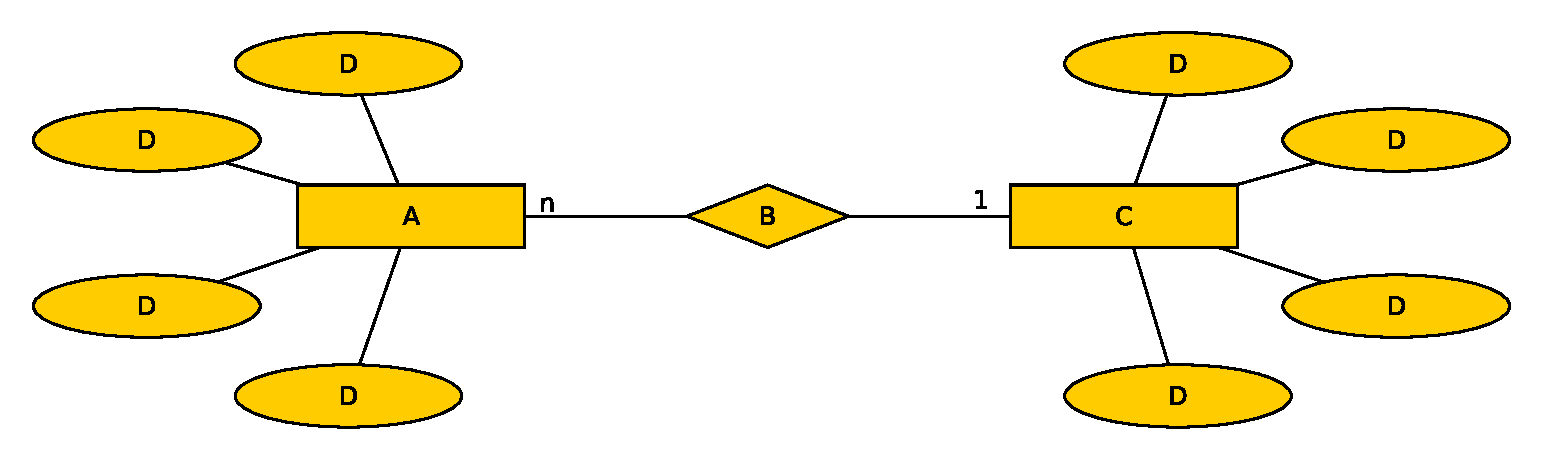
\includegraphics[scale=0.6, ]{EntityBeis.pdf}
	\label{fig:eBeis}
	\end{center}
	
	\paragraph{Attribut (D)} In dieser Grafik werden die Attribute bzw. Domänen durch Ellipsen dargestellt. In einer Bildlichen darstellen durch Tabellen würden Domänen die Spaltenüberschriften repräsentieren. Eine Domäne kann als Primary Key für eine Entitätsmenge gekennzeichnet werden. Dies geschieht, indem man den Domänenamen unterstreicht\footnote{vgl. \cite{Jarosch2010} 7.5 Datenbankentwurf: Attribut}.
	
	\paragraph{Entitätsmenge (A, B)} Die Entitätsmengen werden durch Vierecke dargestellt. Im übertragenen Sinne sind dies Tabellen. Entitätsmengen sind von Attributen umringt. Davon ist normaler Weise mindestens eines ein Primary Key\footnote{vgl. \cite{Jarosch2010} 7.5 Datenbankentwurf: Entität}.
	
	\paragraph{Beziehungsmenge (B)} Eine Raute beschreibt eine Beziehungsmenge1. In der Mitte steht die reale Beziehung zwischen den Entitätsmengen z.B. „besitzt“ oder „ist in“. Die Raute ist mit zwei Strichen mit den zugehörigen Entitätsmengen verbunden.  Auf diesen Pfeilen werden die Kardinalitäten notiert. Dabei steht die Menge der Beziehungen einer einzelnen Entität auf der anderen Seite der Raute. In dem abgebildeten Beispiel kann eine Zeile in A nur auf einen Zeile in C verweisen, aber eine Zeile in C kann auf beliebig viele Zeilen in A verweisen\footnote{vgl. \cite{Jarosch2010} 7.5 Datenbankentwurf: Beziehung}. 
	
	\subsection{Datenbank erstellen}
	\label{sec:dbErst}
	Die in \ref{sec:dbArten} besprochenen Unterschiede sprechen klar dafür, dass ich eine SQLite Datenbank verwenden sollte. Aber, da ich mehr Erfahrung in MySQL habe, habe ich beides gemacht. Die SQL-Befehle habe ich in der offiziellen MySQL-Dokumentation nachgeschaut\footnote{vgl. \cite{sqlDocu}}. Da SQLite auch mit SQL funktioniert konnte ich die Befehle im Grunde übernehmen. \\ 
	\\
Das erste was ich gemacht habe ist eine neue Datenbank zu erstellen. In SQLite ist dies nicht nötig, da es nur einen Datenbank gibt. Damit es keine Zeichenfehler gibt habe ich "u gegen ue ersetzt.
	\begin{lstlisting}[ language=SQL,
	                    deletekeywords={IDENTITY},
	                    deletekeywords={[2]INT},
	                    morekeywords={clustered},
	                    framesep=8pt,
	                    xleftmargin=40pt,
	                    framexleftmargin=40pt,
	                    frame=tb,
	                    framerule=0pt ]
CREATE DATABASE schueler;
	\end{lstlisting}
Danach konnte ich mit der ersten Tabelle beginnen. Für die länge des Vorname und des Nachnamens habe ich 100 Zeichen gewählt. Der Stufenname kann nur aus 2 Buchstaben bestehen, also habe ich ihn darauf auch begrenzt. Die SID wird in MySQL automatisch definiert. In SQLite funktioniert das leider nicht. Also habe ich das Problem gelöst indem ich die SID in SQLite manuel definiere. Somit konnte ich das 'AUTO INCREMENT' Attribute weglassen.
	\begin{lstlisting}[ language=SQL,
	                    deletekeywords={IDENTITY},
	                    deletekeywords={[2]INT},
	                    morekeywords={clustered},
	                    framesep=8pt,
	                    xleftmargin=40pt,
	                    framexleftmargin=40pt,
	                    frame=tb,
	                    framerule=0pt ]
CREATE TABLE schueler(
	SID INT PRIMARY KEY AUTO_INCREMENT, 
	vorname VARCHAR(100), 
	nachname VARCHAR(100), 
	stufe VARCHAR(2)
);
	\end{lstlisting}

Das Erstellen der anderen Tabellen erfolgte mit dem gleichem Befehl. Nur die Arttribute und der Name mussten verändert werden.

	\begin{lstlisting}[ language=SQL,
	                    deletekeywords={IDENTITY},
	                    deletekeywords={[2]INT},
	                    morekeywords={clustered},
	                    framesep=8pt,
	                    xleftmargin=40pt,
	                    framexleftmargin=40pt,
	                    frame=tb,
	                    framerule=0pt ]
CREATE TABLE stunden(
	StId INT AUTO_INCREMENT PRIMARY KEY, 
	vonS INT, 
	bisS INT, 
	tag INT, 
	oft INT
);

CREATE TABLE lehrer(
	short VARCHAR(3) PRIMARY KEY,
	vorname VARCHAR(100), 
	nachname VARCHAR(100),
);

CREATE TABLE kurse(
	name VARCHAR(10), 
	stufe VARCHAR(2), 
	fach VARCHAR(50), 
	art VARCHAR(30),
	nummer INT,
	raum VARCHAR(10), 
	lShort VARCHAR(3), 
	PRIMARY KEY(name, stufe), 
	FOREIGN KEY (lShort) REFERENCES lehrer(short)
);
	\end{lstlisting}
Die Tabellen, die jetzt noch fehlen sind die Beziehungstabellen. Bei diesen ist es wichtig, dass die alle Domänen Foreign Keys und gleichzeitig Primary Keys sind. Da es mehrere Primary Keys gibt müssen diese, genau wie die Foreign Keys, am Ende definiert werden.
	
		\begin{lstlisting}[ language=SQL,
	                    deletekeywords={IDENTITY},
	                    deletekeywords={[2]INT},
	                    morekeywords={clustered},
	                    framesep=8pt,
	                    xleftmargin=40pt,
	                    framexleftmargin=40pt,
	                    frame=tb,
	                    framerule=0pt ]
CREATE TABLE stundenKurs(
	name VARCHAR(10), 
	stufe VARCHAR(2), 
	StId INT, 
	PRIMARY KEY (name, stufe, StId),
	FOREIGN KEY (name, stufe) REFERENCES kurse(name, stufe), 
	FOREIGN KEY (StId) REFERENCES stunden(StId)
);

CREATE TABLE schuelerKurs(
	SID INT, 
	name VARCHAR(10), 
	stufe VARCHAR(2),
	PRIMARY KEY (SID, name, stufe),
	FOREIGN KEY (name, stufe) REFERENCES kurse(name, stufe), 
	FOREIGN KEY (SID) REFERENCES schueler(SID)
);
	\end{lstlisting}
Damit ein Programm von meinem Computer auf den SQL-Datenbankserver zugreifen kann habe ich einen neuen Beutzter erstellet. Diesem musste ich dann die Benutztungsrechte für die meine Datenbank geben. Das ging mit dem folgendem Befehl:
	
	\begin{lstlisting}[ language=SQL,
	                    deletekeywords={IDENTITY},
	                    deletekeywords={[2]INT},
	                    morekeywords={clustered},
	                    framesep=8pt,
	                    xleftmargin=40pt,
	                    framexleftmargin=40pt,
	                    frame=tb,
	                    framerule=0pt ]	
CREATE USER "schueler"@"%" IDENTIFIED BY "stundenplan#1Pas";

GRANT ALL PRIVILEGES ON schueler.* TO schueler;
	\end{lstlisting}	
	In SQLite gibt es nur einen User, deswegen war dies bei der SQLite-Datenbank nicht nötig.
	\subsection{Datenbank füllen}
	Um die Datenbank zu füllen habe ich für jede Tabelle ein Script programmiert. Diese liest eine csv-Datei aus und überträgt jede Zeile in die entsprechende Datenbank. Die csv-Dateien habe ich folgendermassen erstellen:
	\paragraph{Kurse} Ich habe mir aus unserem Kursplan, ein paar Kurse ausgesucht und diese per Hand in das Dokument geschrieben.
	\paragraph{Lehrer} Hier konnte ich die Kürzelliste von der Schulwebsite Kopieren und dann mit einem Script in die gewünschte Form bringen.
	\paragraph{Sch"uler} Die Namen in dieser Tabelle sind frei erfunden.
	\paragraph{Sch"ulerKurs} Da die Namen schon frei erfunden waren war es schwer für diese eine Kursbelegung zu finden. Also habe ich mir auch eine Ausgedacht und versucht keine Zeiten doppelt zu belegen.
	\paragraph{Stunden} Ich habe einfach alle möglichen Kurszeiten per Hand abgeschrieben.
	\paragraph{StundenKurs} Hier habe ich per Hand die entsprechden Zeiten aus dem Kursplan abgeschrieben.
	\subsection{Datenbank auslesen}
	Um die Tabelle auszulesen habe ich für die verschiedenen Anwendungen folgende Befehle konstruiert:
	\paragraph{Kurslisten} \label{sec:selKursLi} Damit man alle Teilnehmer eines Kurses anzeigen kann muss mann zu erst die Schüler Tabelle mit der Schueler-Kurs Tabelle verbinden. Dies geschieht durch den Befehl 'JOIN'. Der Parameter 'ON' beschreibt Wann die Tabellen verbunden werden sollen. In diesem Fall wenn die SID in der Schüler Tabelle gleich mit der SID in der Schüler-Kurs Tabelle ist. Dieser Befehl würde eine Tabelle mit allen Kurs Namen, ihren Stufen und allen Schülern. Da wir aber genauere bzw. Ausgeschriebene Angaben haben will. Habe ich diese Tabelle mit der Kurs Tabelle verbunden. Dies geschieht wenn der name  und die Stufe gleich sind. In der letzten Zeile wird bestimmt welcher Kurs ausgegeben werden soll. Dies geschieht indem eine ausgabe Bedingung hizu gefügt wird. Somit werden nur die Zeilen ausgegeben in den der Name und die Stufe mit den gegebenen Werten "ubereinstimmt. 
	\begin{lstlisting}[ language=SQL,
	                    deletekeywords={IDENTITY},
	                    deletekeywords={[2]INT},
	                    morekeywords={clustered},
	                    framesep=8pt,
	                    xleftmargin=40pt,
	                    framexleftmargin=40pt,
	                    frame=tb,
	                    framerule=0pt ]	
SELECT schueler.vorname, schueler.nachname
FROM schueler
	JOIN schuelerKurs
	ON schueler.SID = schuelerKurs.SID
	JOIN kurse
	ON schuelerKurs.name = kurse.name AND schuelerKurs.stufe = kurse.stufe
WHERE kurse.name = <Kursname> AND kurse.stufe = <stufe>;
	\end{lstlisting}	
	\paragraph{Zeiten} \label{sec:selZeit}
	Um die Zeiten eines Kurses augeben zu können wird die Kurs Tabelle mit der Stunden-Kurs Tabelle verlichen und die Spalten zusammen gefügt wo der Name des Kurses übereinstimmt. Diese Tabelle wird dann mit der stunden Tabelle zusammen fusioniert wo die StId's "ubereinstimmen. Daraufhin werden nur die Zeilen ausgegebne wo der Name und die Stufe mit der gegebenen Stufe und dem gegebenen Namen ist.
	\begin{lstlisting}[ language=SQL,
	                    deletekeywords={IDENTITY},
	                    deletekeywords={[2]INT},
	                    morekeywords={clustered},
	                    framesep=8pt,
	                    xleftmargin=40pt,
	                    framexleftmargin=40pt,
	                    frame=tb,
	                    framerule=0pt ]	
SELECT stunden.tag, stunden.vonS, stunden.bisS
    FROM kurse
        JOIN stundenKurs
        ON kurse.name = stundenKurs.name
        JOIN stunden
        ON stundenKurs.StId = stunden.StId
    WHERE kurse.name = <name> AND kurse.stufe = <stufe>;
	\end{lstlisting}	
	
	\paragraph{Stundenpl"ane} Die Stundenplanabfrage war mit Abstandt die komplizierteste, da fünf Tabellen miteinander Verbunden werden müssen. Ich habe mit der Sch"uler Tabelle begonnen. Diese habe ich wie in \nameref{sec:selKursLi} mit der Sch"uler-Kurs Tabelle verbunden. Die hervorgehenden Tabelle konnte ich dann wie in \nameref{sec:selZeit} mit der Stunden-Kurs Tabelle und der Stunden Tabelle zusammenführen. Aus dieser Tabelle musste ich dann nur noch die Zeilen, in denen der Vorname und Nachname mit den gegeben übereinstimmt ausgegeben werden.
	\begin{lstlisting}[ language=SQL,
	                    deletekeywords={IDENTITY},
	                    deletekeywords={[2]INT},
	                    morekeywords={clustered},
	                    framesep=8pt,
	                    xleftmargin=40pt,
	                    framexleftmargin=40pt,
	                    frame=tb,
	                    framerule=0pt ]	
    SELECT kurse.name, stunden.tag, stunden.vonS, stunden.bisS
    FROM schueler 
        JOIN schuelerKurs
        ON schuelerKurs.SID = schueler.SID
        JOIN kurse 
        ON schuelerKurs.name = kurse.name AND schuelerKurs.stufe = kurse.stufe
        JOIN stundenKurs
        ON kurse.name = stundenKurs.name
        JOIN stunden
        ON stundenKurs.StId = stunden.StId
    WHERE schueler.vorname = <Vorname> AND schueler.nachname = <Nachname> ORDER BY  stunden.tag;
	\end{lstlisting}	
	\subsection{Mein Script}
	Zur einfachen Anwendung dieser Befehle habe ich ein Script programmiert welches eine einfache UI\footnote{UI - User Interface} bietet. Es heißt select.py und sollte auf dem USB-Stick sein\footnote{Denken Sie daran README.txt zu lesen}.
	\newpage
	\section{Zusammenfassung und Ausblick}
	\label{sec:end}
	\newpage
	\printbibliography	
	\appendix
	
	\newpage
	\section*{Schlusserklärung}
	Hiermit versichere ich, dass ich die vorgelegte Arbeit selbstständig angefertigt, keine weiteren als die angegeben	 Hilfsmittel benutzt und die Stellen der Facharbeit, die im Wortlaut oder im wesentlichen Inhalt aus anderen Werken entnommen sind, mit genauer Quellenangabe kenntlich gemacht habe.\\
	\vspace{4cm}
	Verl, den \today
\end{document}
